\section{Gesichtserkennung} \label{sec:recognition}
\begin{tcolorbox}
	\centerline{\textbf{Lernziele Kapitel~\ref{sec:recognition}}}
	\begin{enumerate}[leftmargin=*,label=\thesection.\arabic*]
		\item Erklären können, wie man die Eigengesichter zur Gesichtserkennung nutzen kann.
	\end{enumerate}
\end{tcolorbox}
Nun wollen wir die Eigengesichter nutzen für eine Gesichtserkennung nutzen.
Wie bereits in der Einleitung erklärt, ist Gesichtserkennung im Grunde eine Klassifizierung.
Hier als Beispiel betrachten wir 8 verschiedene Klassen.
\begin{table}[ht]
	\centering
	\begin{tabular}{|c|c|c|c|}
		\hline
		Daniel Radcliffe & Emma Stone & Emma Watson & Eva Green \\
		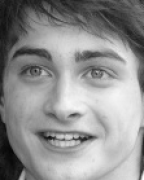
\includegraphics[width=0.2\textwidth]{images/recognition/Daniel_Radcliffe} & 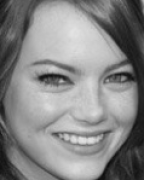
\includegraphics[width=0.2\textwidth]{images/recognition/Emma_Stone} & 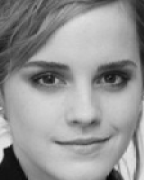
\includegraphics[width=0.2\textwidth]{images/recognition/Emma_Watson} & 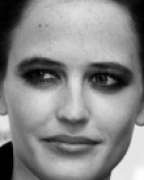
\includegraphics[width=0.2\textwidth]{images/recognition/Eva_Green} \\ \hline
		Jennifer Lawrence & Orlando Bloom & Pierce Brosnan & Tom Cruise \\
		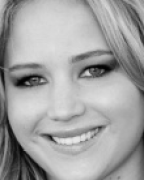
\includegraphics[width=0.2\textwidth]{images/recognition/Jennifer_Lawrence} & 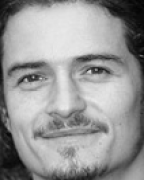
\includegraphics[width=0.2\textwidth]{images/recognition/Orlando_Bloom} & 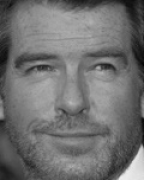
\includegraphics[width=0.2\textwidth]{images/recognition/Pierce_Brosnan} & 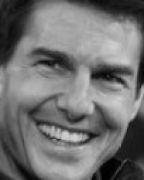
\includegraphics[width=0.2\textwidth]{images/recognition/Tom_Cruise} \\ \hline
	\end{tabular}
	\caption{Die acht verschiedenen Klassen. }
	\label{tab:classes}
\end{table}
Wir verwenden in diesem Kapitel eine Datenbank die nur aus Bilder dieser 8 Personen besteht.
Dabei enthält sie von jeder Person genau 10 Bilder.
Das heisst, sie besteht aus $K=8\cdot 10=80$ Bildern.
Pro Klasse haben wir zusätzlich 3 Testbilder.
Das sind Bilder die zwar jeweils eine dieser 8 Personen zeigen, aber nicht in der Datenbank enthalten sind.
Das Ziel ist nun die Testbilder möglichst der richtigen Klasse zuzuordnen.
So können wir unsere Gesichtserkennung testen, daher der Name \glqq{}Testbilder\grqq{}.
\begin{figure}[ht]
	\centering
	\begin{tabular}{|c m{2cm} m{2cm} m{2cm} m{2cm} m{2cm}|}
		\hline
		Datanbank &
		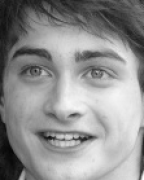
\includegraphics[width=0.1\textwidth]{images/recognition/training_faces/training_0} &
		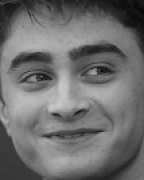
\includegraphics[width=0.1\textwidth]{images/recognition/training_faces/training_1} &
		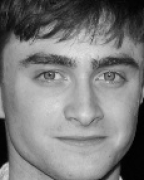
\includegraphics[width=0.1\textwidth]{images/recognition/training_faces/training_2} &
		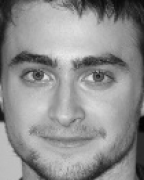
\includegraphics[width=0.1\textwidth]{images/recognition/training_faces/training_3} &
		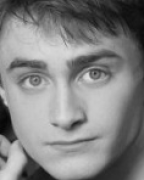
\includegraphics[width=0.1\textwidth]{images/recognition/training_faces/training_4} \\
		&
		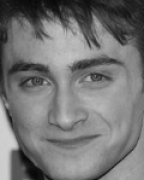
\includegraphics[width=0.1\textwidth]{images/recognition/training_faces/training_5} &
		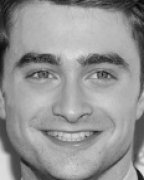
\includegraphics[width=0.1\textwidth]{images/recognition/training_faces/training_6} &
		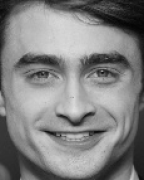
\includegraphics[width=0.1\textwidth]{images/recognition/training_faces/training_7} &
		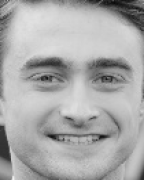
\includegraphics[width=0.1\textwidth]{images/recognition/training_faces/training_8} &
		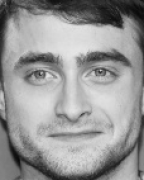
\includegraphics[width=0.1\textwidth]{images/recognition/training_faces/training_9} \\ \hline
		Testbilder &
		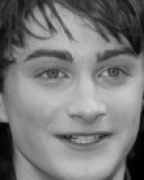
\includegraphics[width=0.1\textwidth]{images/recognition/test_faces/test_0} &
		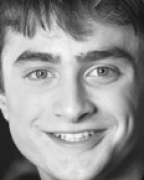
\includegraphics[width=0.1\textwidth]{images/recognition/test_faces/test_1} &
		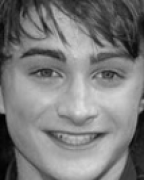
\includegraphics[width=0.1\textwidth]{images/recognition/test_faces/test_2} &
		& \\ \hline
	\end{tabular}
	\caption{Datenbank- und Testbilder am Beispiel der Klasse \glqq{}Daniel Radcliffe\grqq{}}
	\label{fig:testfaces}
\end{figure}
Zwar ist das für einen Menschen ganz leicht, aber für einen Computer ist das überhaupt nicht einfach.
Im Grunde müssen wir den Computer lehren, wann zwei Bilder ähnlich aussehen.
Dazu brauchen wir ein Mass für die Distanz zweier Bilder.
Es stellt sich heraus, dass die Eigengesichter ein Solches liefern.
Seien nun $\vec p$ und $\vec q$ zwei Bilder von Gesichtern.
Wir schreiben die entsprechenden Differenzgesichter als Linearkombination der Eigengesichter
\begin{equation*}
	\vec p-\vec m=c_1\vec u_1+c_2\vec u_2+\ldots+c_K\vec u_K
\end{equation*}
und
\begin{equation*}
	\vec q-\vec m=\tilde c_1\vec u_1+\tilde c_2\vec u_2+\ldots+\tilde c_K\vec u_K,
\end{equation*}
wobei nun $K=80$ und $\vec m$ das Durchschnittsgesicht der Bilder der neuen Datenbank ist.
Entsprechend sehen die Eigengesichter auch etwas anders aus, aber deren Eigenschaften sind die selben.
Das besagte Mass der Distanz zwischen den Gesichtern $\vec p$ und $\vec q$ ist definiert als
\begin{equation*}
	D\left(\vec p,\vec q\right)=\left(c_1-\tilde c_1\right)^2+\left(c_2-\tilde c_2\right)^2+\ldots+\left(c_K-\tilde c_K\right)^2.
\end{equation*}